\section{Harmonic Search}

\subsection{Resumen}

El algoritmo de búsqueda armónica (HS), originalmente propuesto en \cite{hs1}, toma inspiración del proceso de improvisación que sigue un grupo de músicos en busca de la armonía perfecta.
Estos músicos realizan un número de prácticas, improvisando nuevas armonías en cada una de ellas. Cada práctica no comienza desde cero, y es que las improvisaciones pasadas ayudan e influyen en la producción de nuevas armonías de mejor calidad.

\vspace{\baselineskip}

\begin{figure}[H]
    \centering
    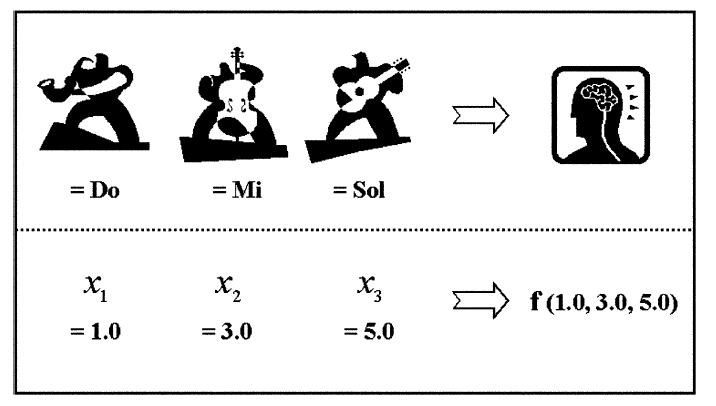
\includegraphics[width=0.55\linewidth]{img/a.png}
    \caption{Inspiración de HS. Imagen tomada de \cite{hs1}}
    \label{a}
\end{figure}

\vspace{\baselineskip}

Tal y como indican los autores en \cite{hs2}, los elementos se extrapolan a una metaheurística de la siguiente manera:
\begin{itemize}
    \item Una armonía está formada por notas, e igualmente una solución candidata está formada a base de variables.
    \item La valoración estética de la armonía se transforma en una evaluación de la función objetivo.
    \item La mejor armonía se convierte en el mejor óptimo.
    \item El cambio de tono se corresponde con variar un elemento de la solución.
    \item Cada práctica (producción de una nueva armonía) se representa como una nueva iteración del algoritmo.
\end{itemize}

\vspace{\baselineskip}

Por tanto, denominamos armonía a una solución candidata del problema \\
$x = \{y_1, y_2, ..., y_n\}$, donde cada $y_i$ representa una nota de la armonía.

\vspace{\baselineskip}

Esta metaheurística hace uso de una estructura de datos, llamada \textbf{harmony memory} (HM), en la cuál se almacenan las armonías ya descubiertas, ordenadas en base a su calidad. De forma similar a un algoritmo generacional elitista, en cada iteración se comparará la nueva solución obtenida con la peor existente en la HM, sustituyéndola en caso de que mejore a la peor existente.

De esta manera el algoritmo pretende paliar los problemas generados por una fuerte convergencia con poca cantidad de exploración. Mediante el uso de la HM permite trabajar con múltiples soluciones al mismo tiempo y no limitar el espacio de búsqueda por culpa de la solución inicial.

\vspace{\baselineskip}

Otro concepto de relevancia para la comprensión del algoritmo es el denominado \textbf{ajuste de tono}. Este es un operador que modifica el valor de una nota una distancia por arriba o por abajo.

\vspace{\baselineskip}

Los parámetros utilizados en el algoritmo son:
\begin{itemize}
    \item \textbf{hms}: Tamaño de la harmony memory (\textbf{HM}).
    \item \textbf{HMCR}: Probabilidad de usar una solución ya existente en la HM.
    \item \textbf{PAR}: Probabilidad de ajustar el tono de un elemento en una nueva armonía. Un PAR de 0.3 indicaría que se elige un vecino con un 30\% * HMCR de probabilidad.
    \item \textbf{bw}: Cantidad de ajuste del tono. Indica cuánto puede mutar un elemento de la solución. Este valor es muy dependiente del problema y de si se están tratando con valores continuos o discretos.
\end{itemize}

\vspace{\baselineskip}

\begin{figure}[H]
    \centering
    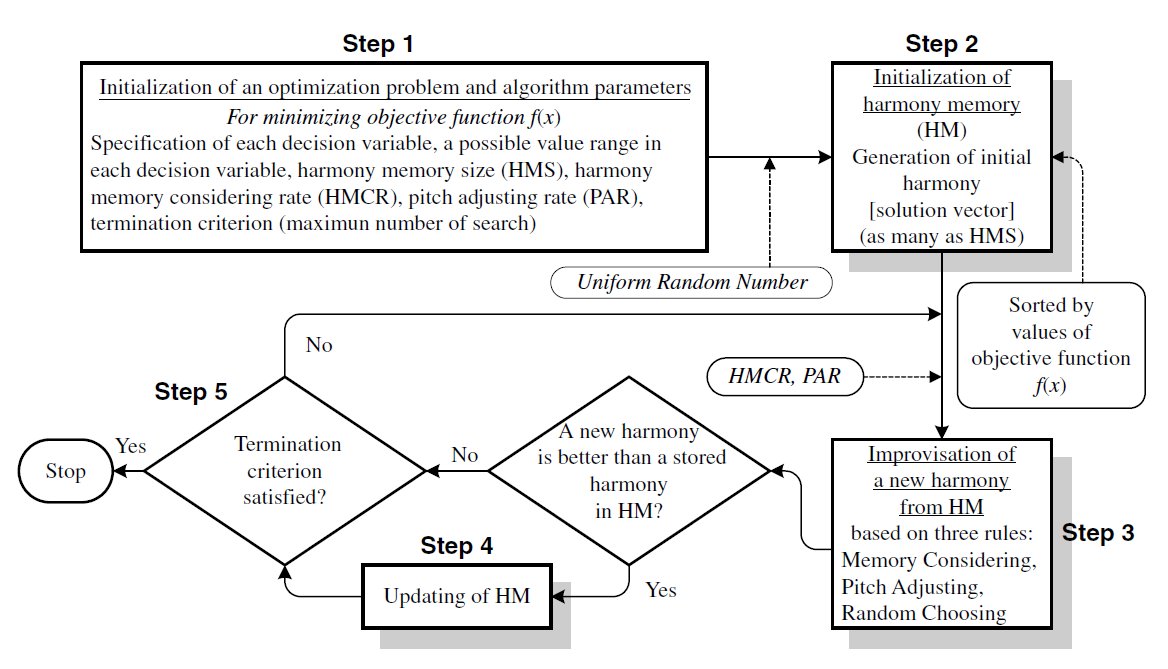
\includegraphics[width=0.95\linewidth]{img/b.png}
    \caption{Proceso de búsqueda en HS. Imagen tomada de \cite{hs1}}
    \label{proceso}
\end{figure}

\vspace{\baselineskip}

El proceso de búsqueda, representado en la figura \ref{proceso}, es el siguiente:
\begin{enumerate}
    \item Inicialización de parámetros y del proceso de búsqueda.
    \item Crear una memoria armónica \textbf{HM} inicial.
    \item Mientras no se cumpla el criterio de parada, repetir:
    \begin{enumerate}
        \item Improvisar una nueva armonía. Para ello repetimos para cada nota:
        \begin{enumerate}
            \item Seleccionar una nota de la HM con probabilidad HMCR, o generar una completamente nueva con probabilidad (1 - HMCR).
            \item Si se ha seleccionado una nota de la HM, aplicar ajuste de tono con probabilidad PAR, y modificado en base al parámetro \textit{bw}.
            
            El ajuste de tono sigue la fórmula: $x_i' = x_i + bw * u(-1, 1)$.

            Donde $u(-1,1)$ es una distribución uniforme entre -1 y 1.
        \end{enumerate}
        \item Actualizar la HM de forma elitista sustituyendo el peor elemento de la tabla por la nueva armonía en caso de que esta lo mejore.
    \end{enumerate}
    \item Devolver la mejor armonía de la HM.
\end{enumerate}

\vspace{\baselineskip}

Queda claro que HMCR y PAR son los parámetros más influyentes en este algoritmo. El primero nos indica la cantidad de exploración en el espacio de búsqueda y el segundo la optimización que se realiza a las soluciones ya encontradas.

\vspace{\baselineskip}

Puesto que el algoritmo no especifica ningún criterio de parada predeterminado, en nuestro caso se adoptará la condición de alcanzar un número de iteraciones fijo.

% ------------------------------------------------------------------------------

\subsection{Mejoras}

El mayor problema que se encuentra es la poca convergencia con la que cuenta. Para solucionarlo se proponen las siguientes alternativas:

\begin{itemize}
    \item Cortar la ejecución en las últimas etapas del algoritmo y aplicar una búsqueda local sobre la mejor solución em la HM. Esta idea nos permite optimizar la solución una vez estamos convencidos de que es prometedora.
    \item Cortar la ejecución en una etapa aún más temprana y aplicar BL sobre las N mejores soluciones en la HM. De esta manera intentamos reducir el impacto de reducir el espacio de búsqueda al no convertirlo en una única solución a optimizar. Para mantener unos costes computacionales comparables, debemos reducir la cantidad de optimización aplicada, tomando el riesgo de no alcanzar completamente el óptimo.
    \item Reducir \textit{hms} (el tamaño de la HM) y aplicar una búsqueda multiarranque del algoritmo.
    \item Modificar los parámetros del algoritmo durante su ejecución. Si reducimos el valor de HMCR durante el proceso de búsqueda, incrementamos la improvisación sobre armonías pasadas reduciendo la exploración en las últimas etapas del proceso de búsqueda. Similarmente modificando PAR de forma variable reducimos la cantidad de optimización introducida. 
    % Es posible que esta aproximación por sí sola no mejore mucho los resultados pero en combinación con alguno de los métodos anteriores sea una buena consideración.
\end{itemize}